\begin{figure}[h]
\centering
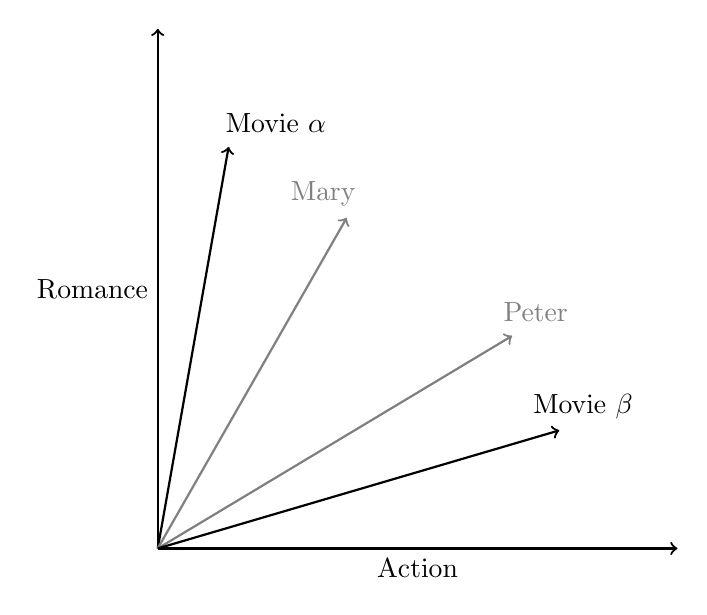
\begin{tikzpicture}[scale=6]
    % Draw the coordinate axes with arrows
    \draw[thick, ->] (0,0) -- (1.1,0);
    \draw[thick, ->] (0,0) -- (0,1.1);
    
    % Place axis labels in the middle of each axis
    \node[below] at (0.55,0) {Action};
    \node[left] at (0,0.55) {Romance};
    
    % Draw arrows and labels
    % Movie α arrow (black, steep upward)
    \draw[black, thick, ->] (0,0) -- (0.15,0.85);
    \node[black] at (0.25,0.9) {Movie $\alpha$};
    
    % Mary arrow (dark gray, medium slope)
    \draw[black!50, thick, ->] (0,0) -- (0.4,0.7);
    \node[black!50] at (0.35,0.75) {Mary};
    
    % Peter arrow (medium gray, moderate slope)
    \draw[black!50, thick, ->] (0,0) -- (0.75,0.45);
    \node[black!50] at (0.8,0.5) {Peter};
    
    % Movie β arrow (light gray, slight upward slope)
    \draw[black, thick, ->] (0,0) -- (0.85,0.25);
    \node[black] at (0.9,0.3) {Movie $\beta$};
\end{tikzpicture}

\caption{An example of a user's movie selection process with hidden variables.}
\label{fig:movie_selection}
\end{figure}